\documentclass[12pt]{article}
\usepackage[a4paper,margin=1.25cm]{geometry}
\usepackage{amsmath,amssymb,mathtools}
\usepackage{graphicx}
\usepackage{booktabs}
\usepackage{tabularx}
\usepackage{tikz}
\usepackage[T1]{fontenc}
\usepackage[utf8]{inputenc}
\usepackage[english]{babel}

\setlength{\parindent}{0pt}
\setlength{\parskip}{0.45em}
\setlength{\abovedisplayskip}{5pt plus 1pt minus 1pt}
\setlength{\belowdisplayskip}{5pt plus 1pt minus 1pt}
\setlength{\abovedisplayshortskip}{3pt plus 1pt minus 1pt}
\setlength{\belowdisplayshortskip}{3pt plus 1pt minus 1pt}

\newcommand{\dd}{\,\mathrm{d}}
\newcommand{\e}{\mathrm{e}}
\newcommand{\In}{I_n}

\begin{document}

\begin{center}
{\Large\bfseries A ratio of truncated logarithmic series}\\[0.35em]
{\large the exponents \(n+1\) and \(n\) cancel against a telescoping sum}
\end{center}

\[
\boxed{\displaystyle
\lim_{n\to\infty}\int_0^1
\frac{\left(1+x+\frac{x^2}{2}+\cdots+\frac{x^{n-1}}{n-1}\right)^{n+1}}
     {\left(1+x+\frac{x^2}{2}+\cdots+\frac{x^{n}}{n}\right)^{n}}
\dd x
=2 .}
\]

\textbf{Overview.}
Write
\[
S_m(x)=1+\sum_{k=1}^{m}\frac{x^k}{k},
\]
so the integrand is \(S_{n-1}^{\,n+1}/S_n^{\,n}\). Two facts settle the
problem, and neither requires any asymptotic analysis.

First, the integrand is \(S_{n-1}\) times \((S_{n-1}/S_n)^n\), and the
second factor is close to \(1\) because the two polynomials differ by the
single term \(x^n/n\). Quantitatively, the defect is bounded by \(x^n\)
uniformly, which integrates to \(\frac1{n+1}\).

Second, \(\int_0^1 S_{n-1}\) telescopes exactly:
\[
\int_0^1 S_{n-1}(x)\dd x=2-\frac1n .
\]
Together these squeeze the integral between \(2-\frac1n-\frac1{n+1}\) and
\(2-\frac1n\), so the limit is \(2\).

\section*{1. Notation and the shape of the integrand}

Set
\[
S_m(x)=1+\sum_{k=1}^{m}\frac{x^k}{k},\qquad m\ge0,\qquad S_0\equiv1 .
\]
For \(x\in[0,1]\) all terms are non-negative, so \(S_m(x)\ge1>0\) and
\(S_m\) is increasing in \(m\). In particular the quotient
\[
r_n(x):=\frac{S_{n-1}(x)}{S_n(x)}\in(0,1]
\tag{1}
\]
is well defined, with \(r_n(0)=1\).

Splitting off one factor of \(S_{n-1}\),
\[
\In:=\int_0^1\frac{S_{n-1}^{\,n+1}}{S_n^{\,n}}\dd x
=\int_0^1 S_{n-1}(x)\,r_n(x)^n\dd x .
\tag{2}
\]
Since \(0<r_n\le1\), we get immediately
\[
0<\In\le\int_0^1 S_{n-1}(x)\dd x .
\tag{3}
\]
Everything now depends on how far \(r_n^{\,n}\) can fall below \(1\).

\section*{2. The defect is bounded by \(x^n\)}

The two polynomials differ by exactly one monomial:
\[
S_n(x)-S_{n-1}(x)=\frac{x^n}{n}.
\tag{4}
\]

\textbf{Lemma.} For all \(x\in[0,1]\) and all \(n\ge1\),
\[
\boxed{\displaystyle
0\le S_{n-1}(x)\bigl(1-r_n(x)^n\bigr)\le x^n .}
\tag{5}
\]

\textit{Proof.} Write \(r=r_n(x)\in(0,1]\). The finite geometric identity
\[
1-r^{\,n}=(1-r)\sum_{j=0}^{n-1}r^{\,j}
\]
gives
\[
S_{n-1}\bigl(1-r^{\,n}\bigr)
=S_{n-1}(1-r)\sum_{j=0}^{n-1}r^{\,j}.
\]
By (1) and (4),
\[
S_{n-1}(1-r)
=S_{n-1}\cdot\frac{S_n-S_{n-1}}{S_n}
=\frac{x^n}{n}\cdot\frac{S_{n-1}}{S_n}
=\frac{x^n}{n}\,r .
\]
Hence
\[
S_{n-1}\bigl(1-r^{\,n}\bigr)
=\frac{x^n}{n}\,r\sum_{j=0}^{n-1}r^{\,j}
\le\frac{x^n}{n}\cdot1\cdot n
=x^n,
\]
because every one of the \(n\) terms \(r^{\,j}\) and the prefactor \(r\)
lie in \((0,1]\). Non-negativity is clear since \(r\le1\). \(\square\)

The lemma is sharp in order: at \(x=1\) one has
\(S_{n-1}(1)=1+H_{n-1}\approx\log n\) and \(1-r_n(1)^n\approx
\frac{1}{n}\cdot\frac{n}{1+H_n}\approx\frac1{\log n}\), so the left side
is of order \(1\), matching \(x^n=1\).

Integrating (5) over \([0,1]\),
\[
0\le\int_0^1 S_{n-1}\dd x-\In\le\int_0^1x^n\dd x=\frac1{n+1},
\tag{6}
\]
that is,
\[
\int_0^1S_{n-1}(x)\dd x-\frac1{n+1}\ \le\ \In\ \le\ \int_0^1S_{n-1}(x)\dd x .
\tag{7}
\]

\section*{3. The telescoping evaluation}

The remaining integral is exact:
\[
\begin{aligned}
\int_0^1S_{n-1}(x)\dd x
&=1+\sum_{k=1}^{n-1}\frac1k\int_0^1x^k\dd x
=1+\sum_{k=1}^{n-1}\frac1{k(k+1)}\\
&=1+\sum_{k=1}^{n-1}\left(\frac1k-\frac1{k+1}\right)
=1+\left(1-\frac1n\right)
=2-\frac1n .
\end{aligned}
\tag{8}
\]
The harmonic-looking coefficients \(\frac1k\) and the integration of
\(x^k\) conspire into the telescoping sum \(\sum\frac1{k(k+1)}\); this is
the only place where the specific coefficients of the series matter, and
it is what produces the answer \(2=1+1\).

Combining (7) and (8),
\[
\boxed{\displaystyle
2-\frac1n-\frac1{n+1}\ \le\ \In\ \le\ 2-\frac1n ,}
\tag{9}
\]
so \(\In\to2\). Moreover (9) gives the rate:
\[
\In=2-\frac1n+O\!\left(\frac1n\right),
\qquad\text{more precisely}\qquad
\left|\In-2+\frac1n\right|\le\frac1{n+1}.
\]

\begin{center}
\small
\renewcommand{\arraystretch}{1.35}
\begin{tabularx}{0.86\textwidth}{@{}lXXX@{}}
\toprule
\(n\) & lower bound \(2-\frac1n-\frac1{n+1}\) & upper bound \(2-\frac1n\) & width \\
\midrule
\(5\)    & \(1.6333\) & \(1.8000\) & \(0.1667\) \\
\(20\)   & \(1.9024\) & \(1.9500\) & \(0.0476\) \\
\(100\)  & \(1.9801\) & \(1.9900\) & \(0.0099\) \\
\(1000\) & \(1.99800\) & \(1.99900\) & \(0.00100\) \\
\bottomrule
\end{tabularx}
\end{center}

\section*{4. What the limit ``ought'' to be, and why the bound is needed}

There is a heuristic that gets the answer instantly and hides the only
real difficulty. For fixed \(x\in[0,1)\),
\[
S_m(x)\longrightarrow 1+\sum_{k=1}^\infty\frac{x^k}{k}=1-\log(1-x),
\]
and
\[
r_n(x)^n=\left(1-\frac{x^n/n}{S_n(x)}\right)^{n}
\longrightarrow1,
\]
because \(x^n\to0\) geometrically. So the integrand converges pointwise
on \([0,1)\) to \(1-\log(1-x)\), and
\[
\int_0^1\bigl(1-\log(1-x)\bigr)\dd x=1+1=2 .
\tag{10}
\]

The heuristic gives the right number, but the convergence is not uniform,
and the limit function is unbounded at \(x=1\) while every
\(\frac{S_{n-1}^{n+1}}{S_n^n}\) is a polynomial quotient, bounded on
\([0,1]\). What happens near \(x=1\) is a genuine competition:
\(S_{n-1}(1)=1+H_{n-1}\to\infty\) like \(\log n\), while \(r_n(1)^n\) is
bounded away from \(1\). The elementary bound (5) is precisely what
controls that boundary layer, and it does so uniformly, with the crude
estimate \(x^n\) whose integral is \(\frac1{n+1}\).

\begin{center}
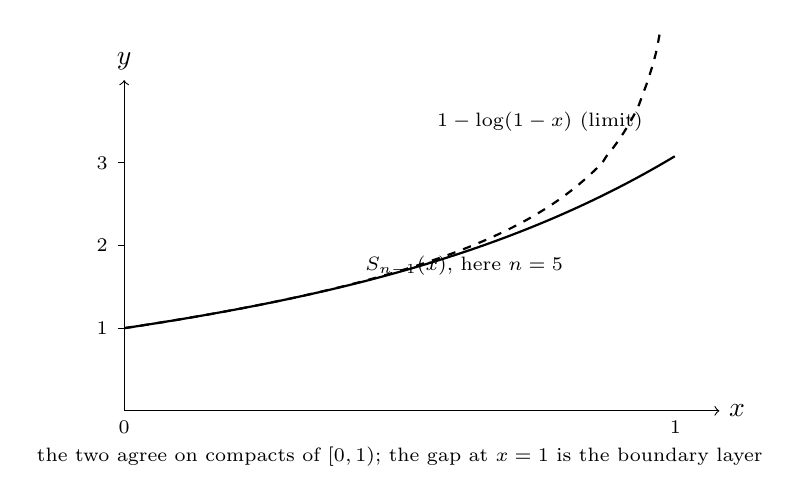
\begin{tikzpicture}[x=7cm,y=1.05cm]
\draw[->] (0,0)--(1.08,0) node[right] {\(x\)};
\draw[->] (0,0)--(0,4.0) node[above] {\(y\)};
\foreach \y in {1,2,3} \draw (0,\y) -- (-0.012,\y) node[left] {\scriptsize \(\y\)};
\node[below] at (0,0) {\scriptsize \(0\)};
\node[below] at (1,0) {\scriptsize \(1\)};
\draw[thick,dashed,samples=120,domain=0:0.975,smooth]
  plot (\x,{1-ln(1-\x)});
\draw[thick,samples=140,domain=0:1,smooth]
  plot (\x,{1+\x+\x*\x/2+\x*\x*\x/3+\x*\x*\x*\x/4});
\node[anchor=west] at (0.55,3.5) {\scriptsize \(1-\log(1-x)\) (limit)};
\node[anchor=west] at (0.42,1.75) {\scriptsize \(S_{n-1}(x)\), here \(n=5\)};
\node[anchor=north] at (0.5,-0.32)
  {\scriptsize the two agree on compacts of \([0,1)\); the gap at \(x=1\) is the boundary layer};
\end{tikzpicture}
\end{center}

Note also that (8) is the finite-\(n\) shadow of (10): the exact value
\(2-\frac1n\) converges to the exact value \(2\) of the limiting
integral, with the discrepancy \(\frac1n\) coming from the truncation of
the series, not from the exponents.

\section*{5. Robustness of the argument}

The proof used three properties of the coefficient sequence
\(c_k=\frac1k\).

\begin{center}
\small
\renewcommand{\arraystretch}{1.45}
\begin{tabularx}{\textwidth}{@{}>{\raggedright\arraybackslash}p{0.30\textwidth}X@{}}
\toprule
Used where & Property \\
\midrule
Lemma, bound \(\frac{x^n}{n}\cdot n\le x^n\)
& The last coefficient satisfies \(c_n\le\frac1n\). Any
\(c_n=O(1/n)\) gives the same conclusion with a constant. \\
\addlinespace
Positivity of \(r_n\le1\)
& \(c_k\ge0\), so \(S_m\) is increasing in \(m\) and bounded below by
\(1\) on \([0,1]\). \\
\addlinespace
Telescoping (8)
& \(\int_0^1x^k\dd x=\frac1{k+1}\) combines with \(c_k=\frac1k\) into
\(\frac1{k(k+1)}\). This is where the value \(2\) is produced. \\
\bottomrule
\end{tabularx}
\end{center}

Consequently, for any non-negative \(c_k\) with \(c_n\le\frac{C}{n}\) and
\(T_m(x)=1+\sum_{k\le m}c_kx^k\),
\[
\lim_{n\to\infty}\int_0^1\frac{T_{n-1}^{\,n+1}}{T_n^{\,n}}\dd x
=1+\sum_{k=1}^{\infty}\frac{c_k}{k+1},
\]
provided the right side converges, by the identical argument. For
\(c_k=\frac1k\) the sum is \(\sum\frac1{k(k+1)}=1\) and the limit is
\(2\); for \(c_k=\frac1{k^2}\) it is
\(1+\sum\frac1{k^2(k+1)}=1+\bigl(\frac{\pi^2}{6}-1\bigr)=\frac{\pi^2}{6}\).

Finally, the mismatched exponents \(n+1\) and \(n\) are a deliberate
distraction. Had they been equal, the integrand would be
\((S_{n-1}/S_n)^n\to1\) and the answer would be \(1\); the extra factor
of \(S_{n-1}\) is the entire content, and once (2) is written down the
problem is about a single polynomial, not a quotient.

\end{document}
